%TODO Spustit program vlna


% Vlozi hlavicku s nastavenim a obecnymi balicky
\documentclass[11pt,a4paper,onecolumn,notitlepage]{article}
\usepackage[czech]{babel}
\usepackage[utf8]{inputenc}
\usepackage{lmodern}
\usepackage[T1]{fontenc}
\usepackage[text={17cm, 24cm},left=2cm,top=3cm]{geometry}
\usepackage{graphicx}
\usepackage{enumitem}
\usepackage[bottom]{footmisc}
\usepackage{xstring}

\usepackage{float}

\floatstyle{plain}
\newfloat{plaintext}{htp}{lop}

\usepackage{xfrac}

\usepackage{color}
\usepackage[unicode,colorlinks,hyperindex,plainpages=false,pdftex]{hyperref}
\usepackage[all]{hypcap}

\graphicspath{ {./img/} }


\providecommand{\todo}[1]{\section{[TODO] #1}}


% Jméno předmětu
\newcommand\courseShortcut{GMU}
\newcommand\courseName{Grafické a multimediální procesory}
\newcommand\projectName{Příprava na zkoušku}



\begin{document}
	
\includegraphics{FIT.pdf}

\begin{center}
	\vspace{\stretch{0.382}}
	\LARGE
	\courseName\ (\courseShortcut)\\
	\Huge
		\projectName\\
	\vspace{\stretch{0.618}}
	\normalsize
	\url{https://github.com/VasaMM/GMU-otazky}
	\hfill
	\today
\end{center}


\pagenumbering{gobble}


\newpage
\pagenumbering{arabic}
\tableofcontents
\newpage




\section{Popište základní principy návrhu energeticky úsporného procesoru CPU/GPU, jak se vyhodnocuje energetická úspornost.}
	Vyhodnocuje se pomocí poměru MFLOPS/W
	
	\begin{itemize}
		\setlength\itemsep{0em}
		\item další snižovaní napájecího napětí není možné
		\item energie na operaci se snižuje lineárně s rozměry prvku
		\item současné technologie 3 W pro mobilní zařízení, 150 W stolní pc
		\item v klasické jednovláknové architektuře se většina energie spotřebuje na režii dodání dat (načtení operandů spotřebuje více E než operace)
		\item Řešení úpravou výpočetní aritmetiky
			\begin{itemize}
				\setlength\itemsep{0em}
				\item Snížení přesnosti kódu čísel, např. odseknutím $n$ nejnižších bitů
				\item přibližné počítání je samostatný specializovaný obor
			\end{itemize}			
		\item Řešení lokalitou dat
			\begin{itemize}
				\setlength\itemsep{0em}
				\item energeticky efektivní architektury musí snížit objem dat přenesených na instrukci
				\item např. přístup do mimočipové paměti $250\times$ dražší
				\item požadavek ma zvýšení šířky pásma paměti mimo čip a snížení příkonu komunikace
			\end{itemize}	
	\end{itemize}
	

\todo{Popište vývoj 2D/3D grafického řetězce s různým stupněm zřetězení.}
	GMU 02
	\begin{figure}[h]
		\centering
		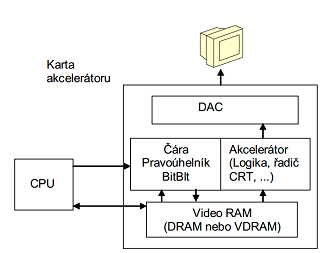
\includegraphics[width=0.6\textwidth]{ZakladniKarta.png}
		\caption{Základní 2D zpracování (IBM 8514)}
		\label{fig:ZakladniKarta}
	\end{figure}

	\begin{figure}[h!]
		\centering
		\includegraphics[width=0.8\textwidth]{ackey.png}
		\caption{Akeleyho pipeline}
		\label{fig:ackey}
	\end{figure}
	generovanie $\rightarrow$ traverzacia $\rightarrow$ transformacia $\rightarrow$ rasterizadia $\rightarrow$ zobrazenie (display) Implementovana napr. u i740, Savage3D


\section{Popište 1- až n-rozměrné multiprocesorové propojovací struktury (Origin/Onyx) a typy propojovacích sběrnic Silicon Graphics.}
	\subsection*{Origin}
		Propojovací struktura architektury koncepce Origin2000 umožnuje vytváret až 5D krychle. Díky její pružnosti a koncepcní pokrokovosti byla prevzata i do navazujících architektur SGI, jako napríklad Onyx2, a další.
		
		Architektura Origin2000 je tvorena množstvím výpoctových uzlu, propojených navzájem propojovací sítí CrayLink. Každý výpoctový uzel obsahuje jeden nebo dva procesory s pametí cache, sdílenou pamet, adresár pro rízení koherence cache s hlavní pametí a dve ruzné jednotky interface – jeden, XIO, který pripojuje I/O jednotky, a druhý, CrayLink, propojující uzly pres jednotku Router.

	\subsection*{Onyx2}
		Každý procesor je spolu se svou pamětí cache a částí operační paměti počítače (o kapacitě od 128 MB do 8 GB) součástí jednoho procesorového uzlu, který obsahuje čtyři procesory. Obousměrný přenos dat mezi procesory v jednom uzlu dosahuje hodnoty 1,6 GBs-1, resp. 800 MBs-1 v každém směru zvlášť. Jednotlivé uzly jsou mezi sebou propojeny pomocí propojovací sítě, jejíž topologie sice vychází z ideální hyperkrychle, ale z důvodu optimalizace datových přenosů jsou mezi uzly vytvořeny i další přídavné datové spoje (již z principu musí jít o diagonály), zejména mezi procesory a zobrazovacími subsystémy.
	

\section{Popište principy výstavby, činnosti a použití GPGPU.}
	Jde o techniku využití GPU k obecným (negrafickým) výpočtům, které běžně probíhají na CPU. Zatímco dříve bylo zpracování dat na GPU pevně dané (static pipeline), dnes už je převážná část programovatelná, a tudíž nabízí možnost obecných výpočtů. K tomu slouží např. rozhraní OpenCL, CUDA či ATI Stream.
	
	Z povahy grafických čipů vychází také způsob práce s daty, který je silně orientován na paralelní proudové zpracování dat. Data jsou často rozdělena do 2D mřížky, kde nad každou buňkou pracuje jedna výpočetní jednotka. Tyto jednotky sdílí kód programu, nazývaný také kernel. Možnost synchronizace či sdílení dat mezi jednotkami v průběhu výpočtu je omezená a značně snižuje výsledný výkon. (Alespoň v OpenCL možnost sdílení paměti existuje.) Z běžných součástí GPU lze použít například texturovací jednotky jako vstupní rozhraní a framebuffer jako výstupní.
	
	Syntaxe programovacího jazyka může být podmnožinou jazyka C (v OpenCL), ovšem existují omezení plynoucí právě z paralelního proudového zpracování. Není možné používat rekurzi, volání vnořených funkcí má svá omezení, jsou zavedeny speciální funkce a datové typy pro práci s vektory, je žádoucí znovuvyužívat použité proměnné a obecně musí optimalizace probíhat jinak než u běžných (CPU) programů - s ohledem na povahu HW.
	
	Vhodnými úlohami pro zpracování na GPU je například zpracování videa, zvuku či řeči, provádění fyzikálních simulací (kapaliny, osvětlení, počasí) anebo třeba úlohy z kryptografie.


\section{Popište koncepci a vlastnosti různých typů Streaming Multiprocesoru}
	Většinu plochy čipu GPU zabírá velké množství relativně jednoduchých skalárních procesorů, případně jednotek VLIW, které jsou organizovány do větších celků zvaných \emph{streaming multiprocesory}.
	Vzhledem k tomu, že se jedná o architekturu SIMT, řízení jednotek a plánování instrukcí je jednoduché a spolu s velmi malou vyrovnávací pamětí zabírá malé procento plochy GPU čipu.
	\begin{figure}[h!]
		\centering
		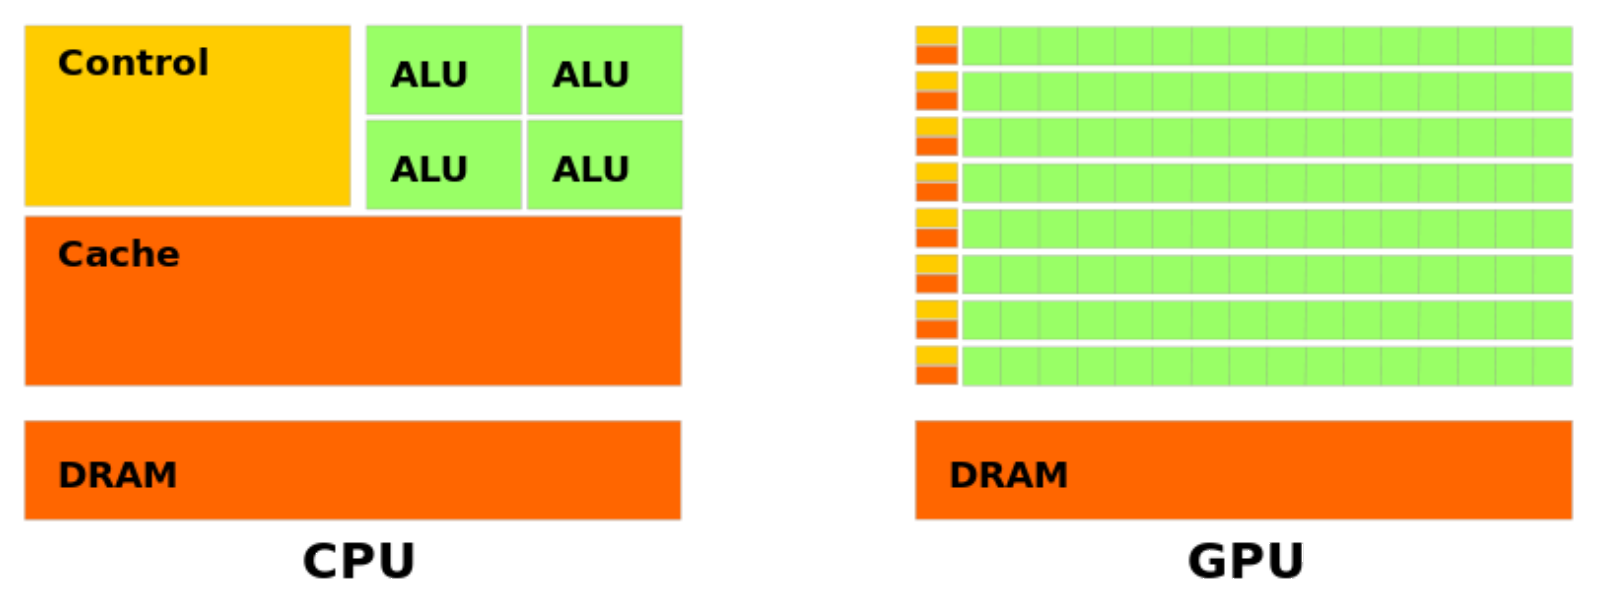
\includegraphics[width=0.8\textwidth]{cpu_vs_gpu.png}
		\caption{Porovnání struktury CPU a GPU}
		\label{fig:cpu_vs_gpu}
	\end{figure}
	
	
\section{Popište principy komprese dat v systému Pascal (delta-komprese a další).}
	\textbf{Komprese v paměti cache L2} \\
	Jsou uplatněny tři principy delta komprese barev. \\
	GPU vypočítává rozdíly mezi barvami pixelů v bloku a ukládá blok jako referenční pixely plus delta hodnoty -- rozdíly od referenčních hodnot. \\
	Pokud jsou delta hodnoty malé, pak je zapotřebí na jeden pixel jen malý	počet bitů. Standardní kompresní metoda vede na kompresní poměr 2:1. \\
	GeForce GTX 1080 Pascal zavedla tyto kompresní režimy:
	\begin{itemize}
		\setlength\itemsep{0em}
		\item Zdokonalená komprese 2:1
		\item Komprese 4:1 pro případ velmi malých hodnot delta
		\item Kompresní režim 8:1 kombinuje kompresi konstantních barev 4:1 pro bloky 2x2 pixelů s kompresí 2:1 hodnot delta mezi těmito bloky
	\end{itemize}	
	
	
\todo{Popište architekturu grafických multiprocesorů a nové principy činnosti, jako komprese dat, preempce a její typy.}
	
	
\section{Popište princip tensorového jádra Turing, k čemu slouží, jaké formáty dat se používají.}
	tensory -- veličiny, dané např. třemi nebo čtyřmi vektory
	
	\subsection*{Princip činnosti tensorového jádra}
	\begin{itemize}
		\setlength\itemsep{0em}
		\item Používané neuronové sítě mají tisíce vrstev a milióny neuronů.
		\item Pro jejich rychlé trénování a dedukování je zapotřebí vysoký výpočetní výkon.
		\item Zde jsou základními operacemi násobení matice – matice (Matrix-Matrix multiplication GEMM).
		\item Používají se k násobení velkých matic vstupních dat a vah v propojených vrstvách sítě.
		\item Násobení matic se provádí v některých aplikacích v jednoduché přesnosti.
		\item Pro trénování a dedukci se používá poloviční přesnosti.
		\item V jádře Volta se používá smíšené přesnosti, násobení matic se vstupy v FP16 a akumulace v FP32.
		\item Tensorová jádra jsou navržena pro činnost s vysokou energetickou efektivností.
	\end{itemize}

	Každé tensorové jádro pracuje s maticemi $4 \times 4$ a provádí operaci Matrix Multiply and Accumulate
	$$D = A \times B + C$$
	kde $A$, $B$, $C$ a $D$ jsou matice $4 \times 4$.
	Vstupy pro maticové násobení $A$, $B$ jsou v FP16, akumulační matice $C$, $D$ mohou být matice FP16 nebo FP32.
	\begin{figure}[h]
		\centering
		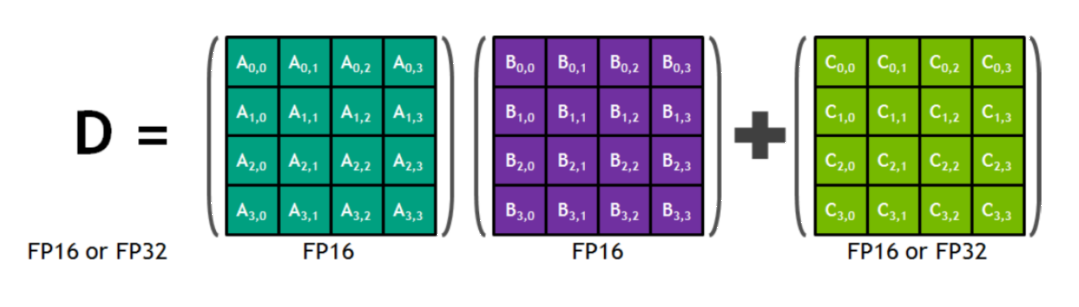
\includegraphics[width=0.8\textwidth]{turing.png}
		\caption{Matrix Multiply and Accumulate}
		\label{fig:turing}
	\end{figure}
	

\section{Popište principy a funkce preempce Pascal.}
	\subsection*{Výpočtová preempce}
		Brání dlouho běžícím aplikacím ovládnout výlučným způsobem celý systém a znemožnit tak běh dalších aplikací, nebo časově překročit.
	
	\subsection*{Preempce pracovní zátěže}
		V zásadě jde o pozastavení vykreslování, uložení kontextu, kde a jak později pokračovat, a rychle přejít na žádost o preempci.

	
	
\section{Popište vývoj unifikovaného adresového prostoru, principy činnosti, a jeho hardwarovou podporu.}
	\begin{itemize}
		\setlength\itemsep{0em}
		\item Programátor nebude muset pracovat s více paměťovými prostory a limitující přenosovou šířkou pásma na paměť a systém bude celkově energeticky úspornější
		\item Společně s koherencí cache zavádí GCN virtuální paměť jako kombinaci hardwarové podpory a driveru
		\item Virtuální paměť GCN je definovaná jako kompatibilní s x86
		\item Tím se zjednoduší přenášení dat mezi CPU a GPU
		\item Dále vytváří možnost bez problémů sdílet jediný adresový prostor pro jednotky CPU i GPU
		\item Sdílení dat bez jejich kopírování je důležitý faktor výkonnosti i příkonové úspornosti v heterogenních systémech
	\end{itemize}
	
	
\section{Popište principy návrhu energeticky úsporného GPU pro mobilní zařízení.}
	\begin{itemize}
		\setlength\itemsep{0em}
		\item V režimu nízké kvality je průměrná kvalita obrázku 26,89 dB s úsporou energie 33,66 \%
		\item V režimu vysoké kvality se dosahuje v průměru 45,94 dB a úspory energie 31,63 \%
		\item Výslednou kvalitu obrázku může vybrat uživatel
		\item Výběr přesnosti se provádí v zásadě automaticky a neovlivňuje vlastní program shaderu
		\item Návrh systému EHPS používá FP se sníženou přesností na 32 bitech a FX na 24 bitech, ALU SIMD a SFU pro úsporu energie
		\item Základní technikou úspory energie v shaderu je používat pevnou řádovou čárku a snížit přesnost čísel s pohyblivou řádovou čárkou
	\end{itemize}
	
	
\todo{Popište hlavní vývojové etapy a principy grafických systémů Mali pro mobilní zařízení.}
	
	
\section{Vysvětlete a zdůvodněte koncepci kachliček (tiles) 16x16 pixelů v grafice Mali.}
	Tento princip je srovnáván s tradičním bezprostředním režimem (immediate mode), používaným typicky v počítačích PC a v terminálech.
	Vykreslování s použitím kachliček znamená vykreslovat buffer snímku z menších úseků -- z kachliček $16 \times 16$ pixelů. Když je kachlička dokončená, vypíše se do paměti.
	
	\subsection*{Bezprostřední režim}
		Vykreslování v bezprostředním režimu se provádí jako přesná posloupnost příkazů pro každý primitiv v každém volání kreslení, nepoužívá se paralelní zpracování a pipelining.
	
	
\todo{Popište formáty dat podporované v grafice Mali, skalární i vektorové.}
	
	
\section{Popište a zdůvodněte principy tří základních typů komprese textur - ztrátové, bezeztrátové a adaptivní.}
	\subsection*{Komprese ASTC}
		Adaptive Scalable Texture Compression je kompresní metoda ARM. Je to ztrátová metoda pro kompresi a dekompresi textur, ukládaných v bufferech v pamětech DDR – Double Data Rate.
		
		Ukládání geometrických dat vyžaduje běžně přes 64 bytů na vrchol, ve srovnání se 4 bity na texel pro Ericsson Texture Compression 2 (ETC2).

	\subsection*{Komprese AFBC}
		ARM Frame Buffer Compression je bezeztrátová kompresní metoda pro kompresi a dekompresi toku videa např. ve formátu H.264. Umožňuje přístup k datům v libovolném místě toku videa.
	
	Metoda AFBC je nyní dostupná pro všechny video stroje Mali, budoucí GPU Mali a jako licencovaný IP pro displejové procesory. 

	
	
\section{Popište alespoň 3 rozdíly mezi architekturami GPU a CPU.}
	\subsection*{CPU}
		\begin{itemize}
			\setlength\itemsep{0em}
			\item programovaní pomocí běžých jazyků (C, C++, \dots)
			\item menší počet komplexních výkoných výpočetních jednotek
			\item predikce skoků, spekulativní vykonávaní, přejmenovaní registrů, vykonývaní instrukcí mimo pořadí, \dots
		\end{itemize}
	\subsection*{GPU}
		\begin{itemize}
			\setlength\itemsep{0em}
			\item programování/konfigurace jednotek pomocí speciálního API (OpenCL, Vulcan)
			\item velké množství jednoduchých skalárních procesorů (SIMD jednotek) organizovaných do desítek multiprocesorů
			\item cca $20\times$ vyšší výkon a $10\times$ paměťová propustnost			
			\item na každý multiprocesor lze naalokovat řádově stovky až tisíce vláken
			\item přepínání vláken bez penalty
			\item různé druhy pamětí sloužící různým účelům
			\item in-order zpracování
		\end{itemize}
	

\section{Co je to kernel?}
	\label{sec:kernel}
	\begin{itemize}
		\setlength\itemsep{0em}
		\item program pro GPU, spouští se paralelně na více vláknech zároveň
		\item sdružuje se do pracovních skupin
		\item typicky definován v externím kódu (OpenGL, OpenCL), spouští se pomocí API
		\item lze jej řadit do front
	\end{itemize}


\section{Co je to vlákno?}
	\begin{itemize}
		\setlength\itemsep{0em}
		\item jedna instance kernelu (viz \ref{sec:kernel})
		\item jsou organizovány do pracovních skupin
		\item každé vlákno má svůj index v rámci skupiny i v rámci kernelu -- slouží k indexaci dat, nad kterými má pracovat (až 3D index)
	\end{itemize}
	

\section{Co je to divergence vláken a kdy vzniká?}
	Když se vlákna jednoho warpu dostanou do různých větví kódu -- toto zpomaluje vykonávání programu, protože jednotlivé větve nelze vykonávat najednou (SIMD ne MIMD)
	a musí se provádět postupně.
	
	Ideálně potřebujeme aby vlákna dělala vždy tu samou instrukci, pokud ne, dochází k divergenci.
	

\section{Co je to warp/wavefront?}
	\begin{itemize}
		\setlength\itemsep{0em}
		\item Skupina vláken (podskupina pracovní skupiny) která patří do jedné pracovní skupiny a vykonávají se společně ve stejnou dobu na jednom multiprocesoru.
		\item Nvidia -- \emph{warp}, AMD -- \emph{wavefront}
		\item Typická velikost 32 nebo 64
	\end{itemize}
	

\section{Co je to multiprocesor (streaming multiprocessor/compute unit) GPU a k čemu slouží.}
	\begin{itemize}
		\setlength\itemsep{0em}
		\item Jsou to hlavni výpočetní jednotky na GPU které vykonávají kód warpu
		\item Nvidia -- \emph{streaming multiprocessor}, AMD -- \emph{compute unit}
		\item akce běžící na různých MP jsou na sobě nezávislé
		\item na jednom MP může běžet víc warpů, pokud na to stačí zdroje
		\item MP má plánovač, který řeší vyhodnocování warpů
		\item na každý MP lze naalokovat až tisíce vláken a typicky obsahuje až desetitisíce 4 B registrů
	\end{itemize}


\section{Co je to fronta příkazů (command queue)?}
	\begin{itemize}
		\setlength\itemsep{0em}
		\item fronta, ve které jsou řazeny jednotlivá volání kernelů pro GPU
		\item OpneGL nemá přímí přístup ke frontě -- vytváří se automaticky při vytvoření kontextu
		\item OpenCL může mít i více front, které manipulují s buffery, spouští kernelů
		\item Implicitně \emph{in-order} fronta (lze přenastavit)
	\end{itemize}


\todo{Jakým způsobem je možné synchronizovat úlohy ve frontě příkazů s vykonáváním mimo pořadí (out-of-order execution) nebo mezi frontami v OpenCL?}
	Pomocí eventů


\section{Jakým způsobem se eliminuje/zmírňuje dopad aritmetických/paměťových latencí.}
	Pokud nějaké vlákno čeká vlivem latence $\rightarrow$ je místo něj spuštěno jiné vlákno, pokud máme přístup k dostatečnému množství vláken které lze spustit můžeme kompletně vyblokovat efekty latence.


\section{Co je to konflikt banků v lokální paměti a kdy vzniká?}
	Banky jsou malé paměťové elementy (přístup do banky zabere 2 cykly) o velikosti 4 B.Nedojde-li ke konfliktu bank, lze k nim přistupovat současně prostřednictvím \emph{half-warpu}. V rámci celého warpu se jedná o 2 “transakce”, kde jedna je pro dolní a druhá pro horní \emph{half-warp}. Konflikt bank spočívá v tom, že dvě paměťové adresy v rámci half-warpu odkazují do stejné banky. V takovém případě se přístup do bank serializuje a není již současný.


\section{Co je to zarovnaný přístup do paměti?}
	Přístup k datům postupně jak jsou v paměti – je třeba si je takto přichystat aby se vždy přistupovalo k smysluplným datům -– toto umožňuje lépe pracovat s pamětí –- zlepšuje to práci cache a plně se využije načítání větších bloků paměti najednou.
	
	Obvykle se doporučuje zarovnávat paměť podle velikosti cache-line, protože jinak může jeden proces zabrat $\sfrac{2}{3}$ řádku a další po něm následující musí jít přes dvě cache-line a bude pomalejší. Ideálně teda zarovnat na celý řádek i když se mrhá daty. Taky přístup k datům je pak rozumnější (indexy).
	


\section{Popište konstantní/uniformní paměť.}
	viz \ref{subsec:konstantni_pamet}


\section{Popište lokální/sdílenou paměť.}
	viz \ref{subsec:lokalni_pamet}


\todo{K čemu slouží texturovací jednotky?}
	Urychleni prace s texturami, obsahuji operace specificke texturam – asi hlavne interpolaci a mozna i nejakou specifickou praci s pameti.


\todo{Jaké jsou rozdíly mezi bufferem a texturou v OpenCL?}
	Textury budou nejspise vyuzivat texturovaci jednotky
	

\section{Jaký je rozdíl mezi normalizovanými a nenormalizovanými texturovacími koordináty?}
	Nenormalizované jsou v rozsahu $[0, x]$, kde $x$ je velikost obrazu.  \\
	U normalizovaných $[0, 1]$.


\section{Co je to register spilling?}
	Když existuje vice proměnných než je možné udržet v registrech musí se některé proměnné ukládat do paměti.


\section{Jaké jsou způsoby komunikace mezi vlákny ve skupině a mezi skupinami?}
	\subsection*{V rámci skupiny}
	\begin{enumerate}
		\setlength\itemsep{0em}
		\item zápis do lokální nebo globální paměti
		\item synchronizace
		\item čtení z lokální nebo globální paměti
	\end{enumerate}
	%
	Omezení při současném zápisu do stejné proměnné z více vláken -- potřeba atomických instrukcí
	
	\subsection*{Jednosměrná komunikace mezi skupinami}
	\begin{itemize}
		\setlength\itemsep{0em}
		\item pomocí globální paměti
		\item není zaručeno pořadí vyhodnocení pracovních skupin
		\item při současném zápisu do stejné proměnné z více skupin -- potřeba atomických instrukcí
	\end{itemize}


\section{K čemu slouží atomické instrukce? Popište jejich vlastnosti a příklad algoritmu kde je možné je využít.}
	\label{sec:atomicke_instrukce}
	K výlučnému přístupu k daným datům a zabráněním WAR, WAW a podobných paměťových chyb. 
	
	Použití třeba u paralelní redukce (suma, min, max, \dots) kdy všechny vlákna chtějí přičíst svou hodnotu k celkovému výsledku, ale bez výlučného přístupu jeden udělá \texttt{sum += $y_1$} a než zapíše, tak jiný udělá své \texttt{sum += $y_2$} a změní původní hodnotu a opožděný první mu ji přepíše a tím se znehodnotí výsledek.
	

\section{Jaké mohou být příčiny nízké výkonnosti kernelů?}
	\begin{itemize}
		\setlength\itemsep{0em}
		\item slabá obsazenost (occupancy)
		\item aritmetické latence - RAW konflikty
		\item divergence vláken - větvení, cykly
		\item paměťové latence
		\item paměťová propustnosti globální/lokální paměti
	\end{itemize}


\section{Co je to obsazenost multiprocesoru (occupancy), na čem je závislá?}
	Vytíženost multiprocessoru –- čím větší tím lepší, závisí na divergenci vláken a na správném rozložení pracovních skupin
	
	Pro maximální rychlost výpočtů má smysl co největší obsazenost, ale když vlákna nemakají (není pro ně práce) je vhodné uvolnit místo pro jiné, ať se nebrzdí výpočet jiných workgroup a podobně. Vhodné je taky uvažovat nad rozmístěním vláken v rámci multiprocesoru.

	\subsection*{Obsazenost multiprocesoru (occupancy)}
		\begin{itemize}
			\setlength\itemsep{0em}
			\item \% naalokovaných vláken z maximálního počtu
			\item alokovatelných vláken na multiprocesor
			\item čím větší \% tím větší množství aktivních warpu na multiprocesor $\rightarrow$ lepší pokrytí aritmetických či paměťových latencí
			\item vlákna se alokují po celých skupinách
		\end{itemize}
	
	\subsection*{Vliv na obsazenost}
		\begin{itemize}
			\setlength\itemsep{0em}
			\item slabá granularita alokace skupin
			\item příliš velké skupiny $\rightarrow$ velký dopad synchronizačních funkcí
			\item příliš malé množství vlaken/skupinu $\rightarrow$ limitace maximálním množstvím skupin
			\item velikost skupiny $\rightarrow$ na nových GPU lze naalokovat maximálně 16 - 32 skupin
			\item spotřeba registrů na vlákno $\rightarrow$ maximální velikost na nových GPU typicky 64 kb na multiprocesor
			\item spotřeba lokální paměti na skupinu $\rightarrow$ maximální velikost na nových GPU typicky 64kB -- 96kb na multiprocesor
		\end{itemize}


\todo{Co je to aritmetická a paměťová latence?}
	Doba čekání na dokončení paměťových operací a aritmetických operací – načítání dat zpravidla trvá více než jeden takt, podobně tomu bývá u dělení a jiných složitých aritmetických operací.
	
	\subsection*{Aritmetická latence}
	\begin{itemize}
		\setlength\itemsep{0em}
		\item způsobena čtením právě zapsané hodnoty (RAW - read after write konflikt)
		\item u moderních GPU typicky 10 -- 20 cyklů
		\item řešení přeskupením instrukcí -- automaticky pomocí kompilátoru
		\item řešení zpracováním více elementů/thread -- stoupá spotřeba registrů, klesá potřeba aktivních warpů na multiprocesor
	\end{itemize}


\todo{Co je to separabilní filtr a jakým způsobem lze přistupovat k jeho paralelizaci?}
	GMU 06, p. 22
	

\section{K čemu slouží paralelní redukce?}
	Paralelizace cyklu se závislostí na předešlé iteraci při operaci která je asociativní -- jde ze složitosti $O(n)$ na $O(log(n))$
	\begin{figure}[h]
		\centering
		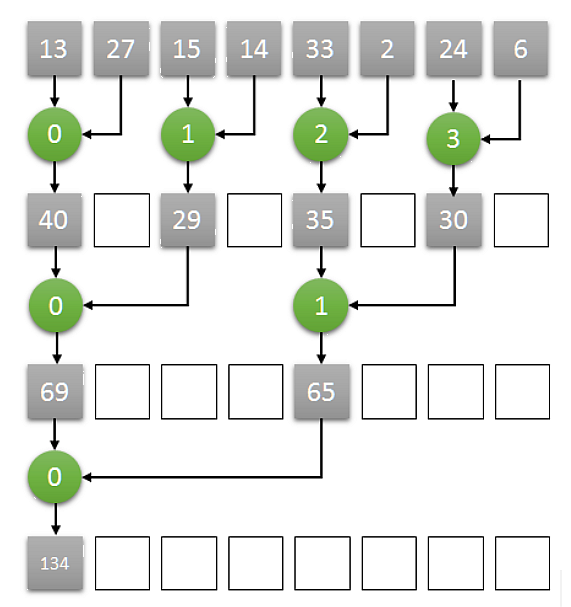
\includegraphics[width=0.6\textwidth]{redukce.png}
		\caption{Příklad paralelní redukce}
		\label{fig:redukce}
	\end{figure}


\section{Co je to dynamický paralelismus?}
	Počet aktivních vláken se mění během výpočtu (došla práce pro některé vlákna, tak je zruším).
	
	Schopnost vlákna kernelu založit další kernel
	

\todo{Jaké jsou možné typy přenosů dat mezi CPU a GPU?}


\section{K čemu slouží P2P přístup a jakým způsobem ho lze využít.}
	Přímý přístup k paměti, používá se hlavně ke zvýšení propustnosti paměti.
	

\section{K čemu slouží operace shuffle?}
	Výměna dat mezi vlákny ve warpu
	\begin{figure}[h]
		\centering
		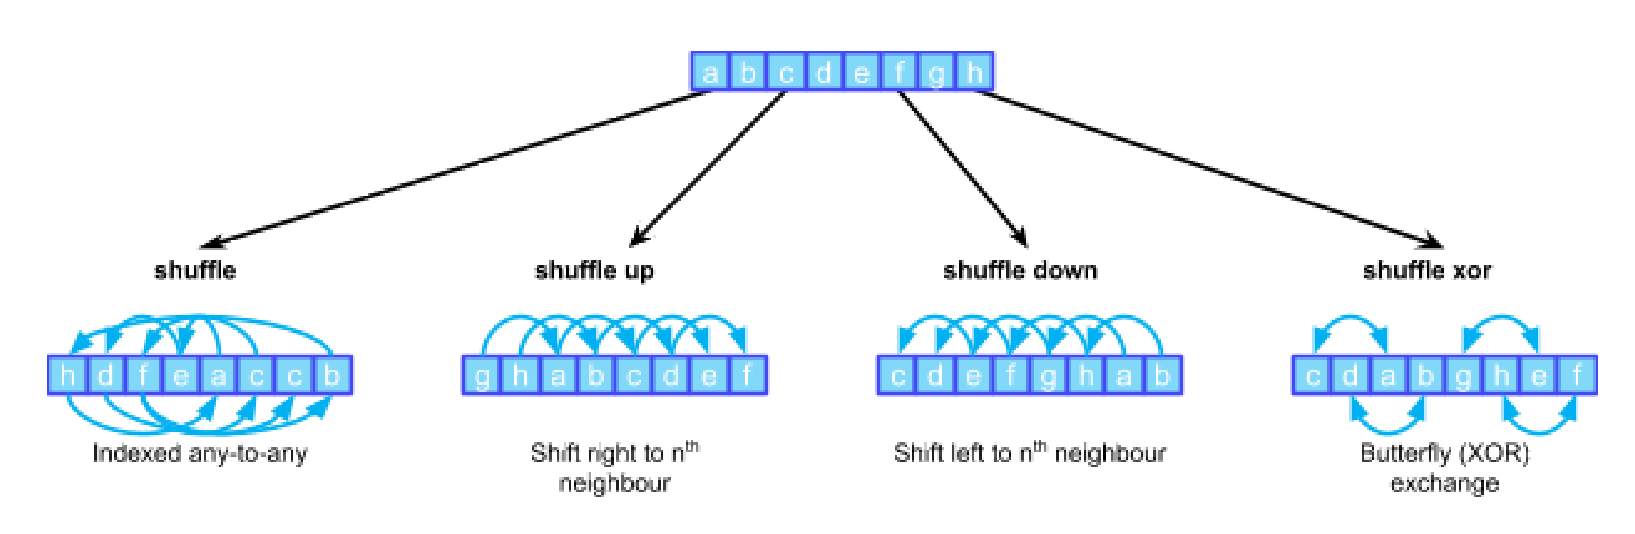
\includegraphics[width=0.6\textwidth]{shuffle.png}
		\caption{Paralelní redukce s shuffle}
		\label{fig:shuffle}
	\end{figure}


\section{Vyjmenujte alespoň 3 api pro GP-GPU.}
	VulkanRT, CUDA, OpenGL, DirectCompute, OpenCL


\section{Co to je SpirV?}
	Softwarový nástroj překládající zdrojové kódy různých platforem (OpenGL, CUDA, \dots) na jednotnou nízkoúrovňovou API. Cílem je zjednodušit vývoj a umožnit použití všeho na všem.
	

\section{K čemu slouží operace ballot?}
	\begin{itemize}
		\setlength\itemsep{0em}
		\item Speciální instrukce \texttt vrací bitovou masku
		\item Umožňuje komunikaci mezi vlákny ve warpu/wavefronte
		\item Každé vlákno ve warpu vyhodnotí podmínku a zapíše	výsledek na bit proměnné jehož číslo odpovídá číslu vlákna ve warpu
		\item \texttt{ballot} instrukce je možná na NVIDIA i AMD
		\item délka warpu je různá (32, 64 bit)
		\item \texttt{ballot} lze simulovat pomocí lokální paměti, ale je to pomalejší
	\end{itemize}


\section{K čemu lze využít atomicCompSwap?}
	viz \ref{sec:atomicke_instrukce}
	
	Instrukci \texttt{atomicCompSwap} lze použít pro implementaci nepodporovaných instrukcí jako jsou například: \texttt{atomicMax}, \texttt{atomicMin}
	
	\texttt{atomicCompSwap(mem, compare, data)} provede atomické porovnání \texttt{mem} a \texttt{compare}. Pokud se rovnají, pak se obsah \texttt{data} zapíše do \texttt{mem}, jinak se nedělá nic. Funkce vrací původní obsah \texttt{mem} bez ohledu na výsledek porovnání.
	
	Možná použití například v řadících algoritmech -- porovnej dvě položky a když jsou opačně, prohoď. (Atomicky proto, aby soused nepracoval s mojí položkou a já neprohodil nesmysl.)	


\todo{Jaký je vztah mezi NDRange/Grid/Dispatch, pracovní skupinou a vláknem/invokací?}
	Pracovní skupina se skládá z vláken

	NDRange (openCL)
	\begin{itemize}
		\setlength\itemsep{0em}
		\item global size -- počet vláken celkově v dané dimenzi
		\item local size - počet vláken v jedné pracovní skupině
		\item počet pracovních grup je určen z global a local size hodnot
	\end{itemize}

	Grid (CUDA) -- 3 dimenze -- počet pracovních grup?

	Dispatch (OpenGL) -- funkce která spustí počet pracovních grup (ve 3 dimenzích) definovaný v jejím volaní?


\section{Jaké paměti jsou na GPU a popište jejich vlastnosti (odkud je lze plnit, odkud je lze číst, relativní rychlost, relativní velikost).}
	\begin{center}
		\begin{tabular}{l|rrrrr}
			\textbf{Typ} & \textbf{Umístšní} & \textbf{Rychlost} & \textbf{Cache} & \textbf{Velikost} & \textbf{Dostupnost} \\ \hline
			global       & off-chip          & 0,11 B/tick        & 1              & $3\;072$ MB           & vše \\
			local        & on-chip           & 1,33 B/tick       & 0              & 0,72 MB           & skupina \\
			constant     & off-chip          & 4 B/tick          & 1              & 64 kB             & vše \\
			register     & on-chip           & 16 B/tick         & 0              & 4 MB              & vlákno                                 
		\end{tabular}
	\end{center}

	\subsection*{Globální paměť}
	\begin{itemize}
		\setlength\itemsep{0em}
		\item off-chip paměť operační paměť grafického adaptéru
		\item velikost v řádech GB
		\item latence v řádu stovek cyklů $\rightarrow$ nutnost běhu mnoha warpůpro překrytí latence (multithreading)
		\item rychlost o řád nižší než on-chip paměti (lokální paměti, registry)
		\item u novějších architektur cachováno pomocí L2 cache, případně i L1 cache $\rightarrow$ zmírnění dopadu opakovaného načítání stejných dat
		\item paměť rozdělena po segmentech
		\item pokud je na jednu adresu ze segmentu přistoupeno z warpu přečte se celý segment
		\item paměťové segmenty se pohybují mezi 32 B a 128 B
		\item u starších architektur nezarovnaný přístup - serializace
	\end{itemize}

	\subsection*{Konstantní paměť}
		\label{subsec:konstantni_pamet}
		\begin{itemize}
			\setlength\itemsep{0em}
			\item lze ji plnit a číst z aplikace
			\item maximální velikost bufferu dle specifikace 64 kb
			\item optimalizace na broadcast $\rightarrow$ přístup do jiných lokací v rámci warpu $\rightarrow$ serializace
			\item cachované pomocí konstatní cache
			\item omezený počet bufferů na kernel -- minimálně 8 dle specifikace
			\item cachování ve speciální cache multiprocesoru
			\item použití: read-only konstanty používané všemi vlákny
		\end{itemize}

	\subsection*{Lokální paměť}
		\label{subsec:lokalni_pamet}
		\begin{itemize}
			\setlength\itemsep{0em}
			\item Sdílená v rámci work-group
			\item Umístěná přímo na čipu -- větší propustnost a menší latence než globální paměť (často se před výpočtem plní z globální paměti)
			\item minimální velikost je pro OpenCL 1.0 16 kB, u novějdšího 32 kB
			\item velikost na předchozích generacích GPU typicky 32 -- 48 kB, na aktuální generaci GPU typicky 64 -- 96 kB
			\item u CPU a některých starších GPU emulovaná pomocí globální paměti -- pomalé, nepoužívat
			\item rozdělena do banků s velikostí buňky typicky 4 B
			\item přístupu do stejného banku více vlákny z warpu -- serializace
			\item novější GPU umějí broadcast a multicast -- přístup z více vláken z warpu na stejnou adresu nezpůsobuje bank konflikty
			\item použití: kooperace mezi vlákny, uživatelské cachování
		\end{itemize}
	
	
	\subsection*{Texturovací paměť}
		\begin{itemize}
			\setlength\itemsep{0em}
			\item data umístěna v globální paměti
			\item 1D až 3D textury
			\item data prochází přes texturovací jednotky $\rightarrow$ interpolace, data mimo rozsah, různé adresování
			\item adresování
			\begin{itemize}
				\setlength\itemsep{0em}
				\item normalizované $\rightarrow$ koordináty staženy do rozsahu $<0{,}0, 1{,}0>$
				\item nenormalizované $\rightarrow$ koordináty v rozsahu $<0{,}0, size>$, první texel na pozici 0,5 $0{,}5$
			\end{itemize}
			\item interpolace
			\begin{itemize}
				\setlength\itemsep{0em}
				\item nejbližší soused $\rightarrow$ zaokrouhlení na nejbližší texel
				\item lineární $\rightarrow$ lineární přechod mezi sousedními texely
			\end{itemize}
			\item řešení okrajů
			\begin{itemize}
				\setlength\itemsep{0em}
				\item opakování obrazu
				\item okrajová hodnota
				\item zrcadlení
			\end{itemize}
			\item optimalizace na načítání bloků
			\item cachování i na starých architekturách, na nových i do L1 cache multiprocesoru
	\end{itemize}

	
	\subsection*{Registry}
	\begin{itemize}
		\setlength\itemsep{0em}
		\item nejrychlejší paměť
		\item přístup do registrů bez latence
		\item typicky desetitisíce 4 B registrů na multiprocesor
		\item pro každé vlákno je alokován potřebný počet registrů -- při příliš velké spotřebě omezuje obsazenost
		\item neblahý vliv na spotřebu registrů může mít rozbalování smyček
		\item příliš mnoho registrů na vlákno $\rightarrow$ register spilling
	\end{itemize}


\section{Jaký je rozdíl mezi pracovní skupinou a warpem/wavefrontem.}
	Oboje jsou skupiny vláken, které spolu mohou komunikovat -- běží na stejné výpočetní jednotce/streaming multiprocessoru
	\subsection*{Pracovní skupina}
		\begin{itemize}
			\setlength\itemsep{0em}
			\item uživatelem definovaná skupina vláken (work-group)
			\item může obsahovat vice wavefrontů –- je jim nadřazená
			\item různé wavefronty mohou vykonávat různé instrukce -- synchronizovat je nutné explicitně
		\end{itemize}
		
	\subsection*{warp/wavefront}
		\begin{itemize}
			\setlength\itemsep{0em}
			\item pro všechna vlákna se vykonává stejná instrukce (při divergency některé ale nemusí pracovat)
		\end{itemize}


\section{K čemu slouží příkaz barrier? Jakou má souvislost s rozdělením vláken do skupin, warpů? Jaký to má vztah k větvení programu?}
	\begin{itemize}
		\item Slouží k synchronizaci vláken
		\item Vlákna můžeme synchronizovat pouze v rámci skupiny (work-groupy)
		\item Synchronizuje se pomocí příkazu \texttt{barrier}
		\item Všechna vlákna ve skupině jej musí zavolat, než kterékoliv může pokračovat
		\item Pokud je \texttt{barrier} v podmínce, musí ji navštívit všechny vlákna ve skupině nebo žádné
		\item V případě, kdyby jedno vlákno vykonávalo jinou \emph{control flow} cestu, ostatní vlákna by zůstaly čekat na \texttt{barrier} donekonečna
	\end{itemize}

	
\end{document}          
